\documentclass[11pt]{article}

\usepackage[a4paper,margin=1in]{geometry}
\usepackage{graphicx}
\usepackage{booktabs}
\usepackage{amsmath}
\usepackage{hyperref}
\usepackage[numbers]{natbib}
\usepackage{enumitem}
\usepackage{float}
\usepackage{setspace}

\onehalfspacing
\graphicspath{{figures/}}
% Auto-generated by run_pipeline.py
\newcommand{\NodeCount}{450}
\newcommand{\TotalSteps}{5500}
\newcommand{\BurnIn}{1000}
\newcommand{\RecordedShocks}{4500}
\newcommand{\ReplicateCount}{5}
\newcommand{\ConnectivityTargets}{1.0, 2.0, 3.0, 4.0, 5.0}
\newcommand{\LargeAvalancheThreshold}{20}
\newcommand{\ConnectivityLow}{1.34}
\newcommand{\ConnectivityMid}{3.02}
\newcommand{\ConnectivityHigh}{4.94}
\newcommand{\MeanAvalancheLow}{0.94}
\newcommand{\MeanAvalancheMid}{1.92}
\newcommand{\MeanAvalancheHigh}{3.05}
\newcommand{\P95AvalancheLow}{3.00}
\newcommand{\P95AvalancheMid}{5.00}
\newcommand{\P95AvalancheHigh}{6.00}
\newcommand{\LargeProbLow}{0.72}
\newcommand{\LargeProbMid}{1.57}
\newcommand{\LargeProbHigh}{2.18}
\newcommand{\VulnerableMid}{30.88}
\newcommand{\MeanGrowth}{3.23}
\newcommand{\LargeProbChange}{1.46}
\newcommand{\HighMaxAvalanche}{424}


\title{Avalanche Dynamics in Software Dependency Networks}
\author{Vishal Gupta}
\date{\today}

\begin{document}
\maketitle

\begin{abstract}
Software package ecosystems are naturally represented as networks of interacting components, which makes them a useful candidate for complexity-science analysis. In this project, a software library is treated as a node in a directed dependency graph, a random developer update is treated as \emph{noise}, and the induced downstream cascade of forced updates is treated as an \emph{avalanche}. I simulate networks containing \NodeCount{} libraries across connectivity targets \ConnectivityTargets{}, using \ReplicateCount{} independent network realizations per regime and \RecordedShocks{} recorded shocks after burn-in in each realization. The results show that avalanche-size distributions broaden as connectivity increases: the mean avalanche size rises from \MeanAvalancheLow{} at low connectivity to \MeanAvalancheHigh{} at high connectivity, while the probability of an avalanche of size at least \LargeAvalancheThreshold{} increases from \LargeProbLow{}\% to \LargeProbHigh{}\%. The network also maintains a persistent near-threshold population of vulnerable libraries, consistent with self-organized near-critical behaviour driven by slow updates and rapid cascade relaxation.
\end{abstract}

\noindent\textbf{Keywords:} complexity science, software dependency networks, avalanches, cascades, self-organized criticality, simulation

\section{Introduction}
Complex systems are often characterised by many interacting components, local rules, feedback, nonlinearity, and emergent large-scale behaviour. Software dependency networks fit this description well. Modern software systems are rarely monolithic; instead, they are assembled from libraries that depend on other libraries. A small local change in an upstream package can therefore propagate through the dependency network and create widespread instability downstream.

This feature makes software dependency ecosystems a useful analogue for complexity-science models of cascading failure. A local update may appear harmless in isolation, but its global consequences depend strongly on the underlying connectivity of the network. This is directly comparable to other complex systems in which local perturbations trigger avalanches, such as sandpiles, power grids, financial contagion, or traffic networks \citep{bak1987,newman2003,albert2002}.

\section{Why This System Is a Good Candidate for Complexity Science}
The chosen system satisfies the main reasons one would apply complexity science:

\begin{enumerate}[leftmargin=1.4em]
\item It contains many interacting units rather than a single dominant control variable.
\item The interaction topology matters: the same update can be harmless in one network and catastrophic in another.
\item Local compatibility rules can generate nonlinear global behaviour.
\item Cascades emerge endogenously from the network structure rather than being programmed as a single global failure rule.
\item The system can exhibit a broad range of event sizes, from negligible local disturbances to large avalanches.
\end{enumerate}

For this reason, a software dependency network is a strong candidate for a complexity-science project even though it is not a chemical engineering example.

\section{System Description: Noise, Avalanche, and Connectivity}
I model the software ecosystem as a directed acyclic graph. An edge $i \to j$ means that library $j$ depends on library $i$. The direction is chosen so that failures propagate downstream from an updated package to its dependents.

\subsection{Noise}
Noise is represented as a random update to a single source package. Each noise event increments the version of one randomly chosen library by one unit. The update itself is slow and local: only one package is perturbed at a time.

\subsection{Connectivity}
Connectivity is controlled by the average number of dependencies per package. Newer libraries attach to older libraries using a preferential attachment rule so that popular packages acquire many dependents. This choice creates hubs and heterogeneity similar to real software ecosystems.

\subsection{Avalanche}
Each library stores the upstream versions that it last validated against. Let $v_i$ be the current version of upstream package $i$ and $\hat{v}_{ij}$ the version of $i$ that downstream package $j$ expects. The accumulated compatibility strain on package $j$ is
\begin{equation}
\sigma_j = \sum_{i \in \mathcal{D}_j} (v_i - \hat{v}_{ij}),
\end{equation}
where $\mathcal{D}_j$ is the set of dependencies of package $j$. Each package also has a finite compatibility buffer $b_j$. When $\sigma_j \geq b_j$, package $j$ is assumed to break and update. That update resets its expected upstream versions and may in turn push more downstream packages over their thresholds. The avalanche size is the number of downstream libraries forced to update after the initial noisy source update.

\section{Simulation Method}
The simulation proceeds as follows:

\begin{enumerate}[leftmargin=1.4em]
\item Construct a dependency network with \NodeCount{} nodes.
\item Assign each node a compatibility buffer that grows mildly with its in-degree.
\item Apply one random update to an upstream library.
\item Propagate the resulting breakage cascade through downstream dependents.
\item Record avalanche size, cascade depth, mean stress ratio, and the fraction of vulnerable libraries.
\item Repeat for \TotalSteps{} update events, discard the first \BurnIn{} as burn-in, and analyse the remaining \RecordedShocks{}.
\end{enumerate}

The model is deliberately stylised. It does not include semantic version numbers, optional dependencies, maintainer intervention, or coordinated release management. The aim is not to reproduce any one real package registry exactly, but to construct a minimal model in which noise, connectivity, and avalanches can be studied cleanly.

\section{Results}

\subsection{Illustrative Cascade}
Figure~\ref{fig:example} shows a representative update cascade. The blue node is the randomly updated source library, while the red nodes are downstream packages that are forced to update after their compatibility buffers are exceeded.

\begin{figure}[H]
\centering
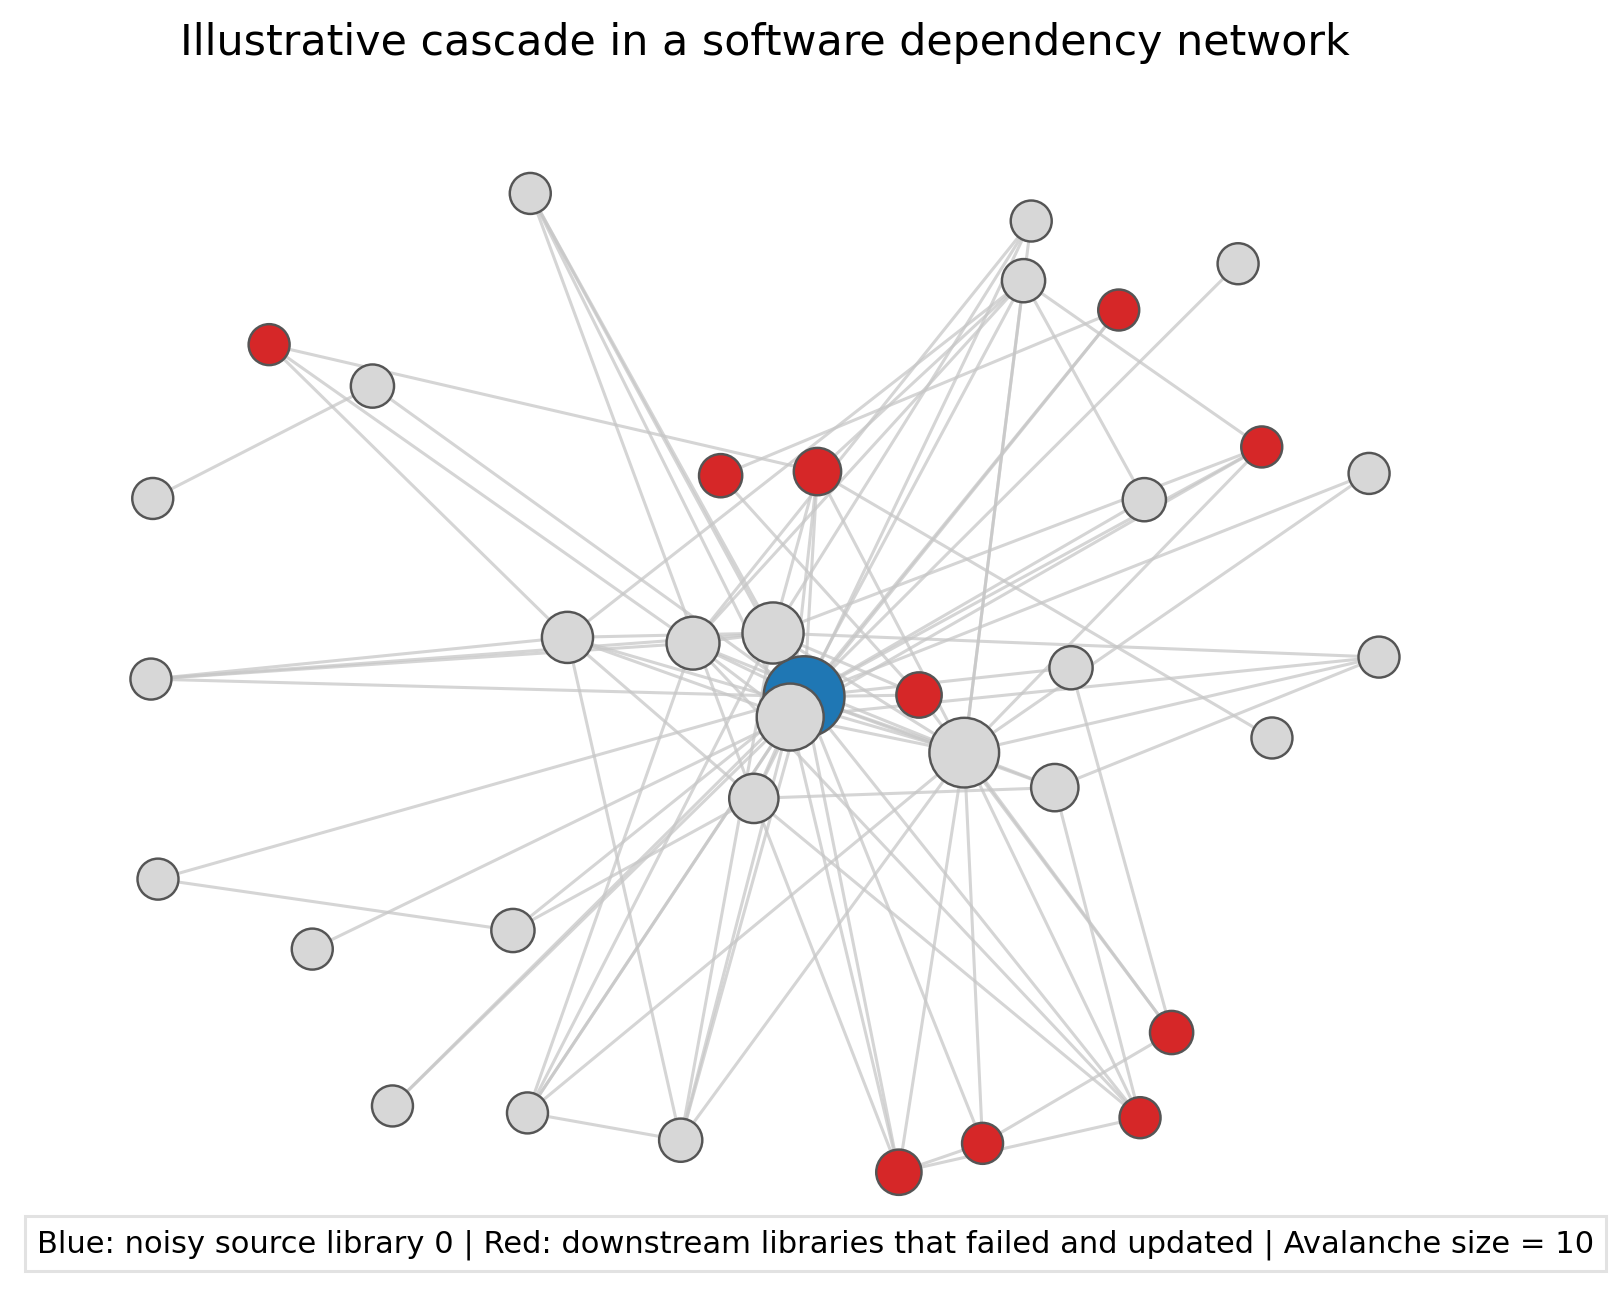
\includegraphics[width=0.82\textwidth]{network_avalanche_example.png}
\caption{Illustrative update avalanche in a software dependency network. A local upstream perturbation propagates through downstream connectivity and causes multiple libraries to fail and update.}
\label{fig:example}
\end{figure}

\subsection{Frequency Distribution of Avalanches}
Figure~\ref{fig:distribution} plots the complementary cumulative distribution of avalanche size for low, medium, and high connectivity regimes. The tail becomes visibly broader as connectivity increases, meaning that denser dependency networks support a wider range of cascade sizes and a larger probability of extreme events.

\begin{figure}[H]
\centering
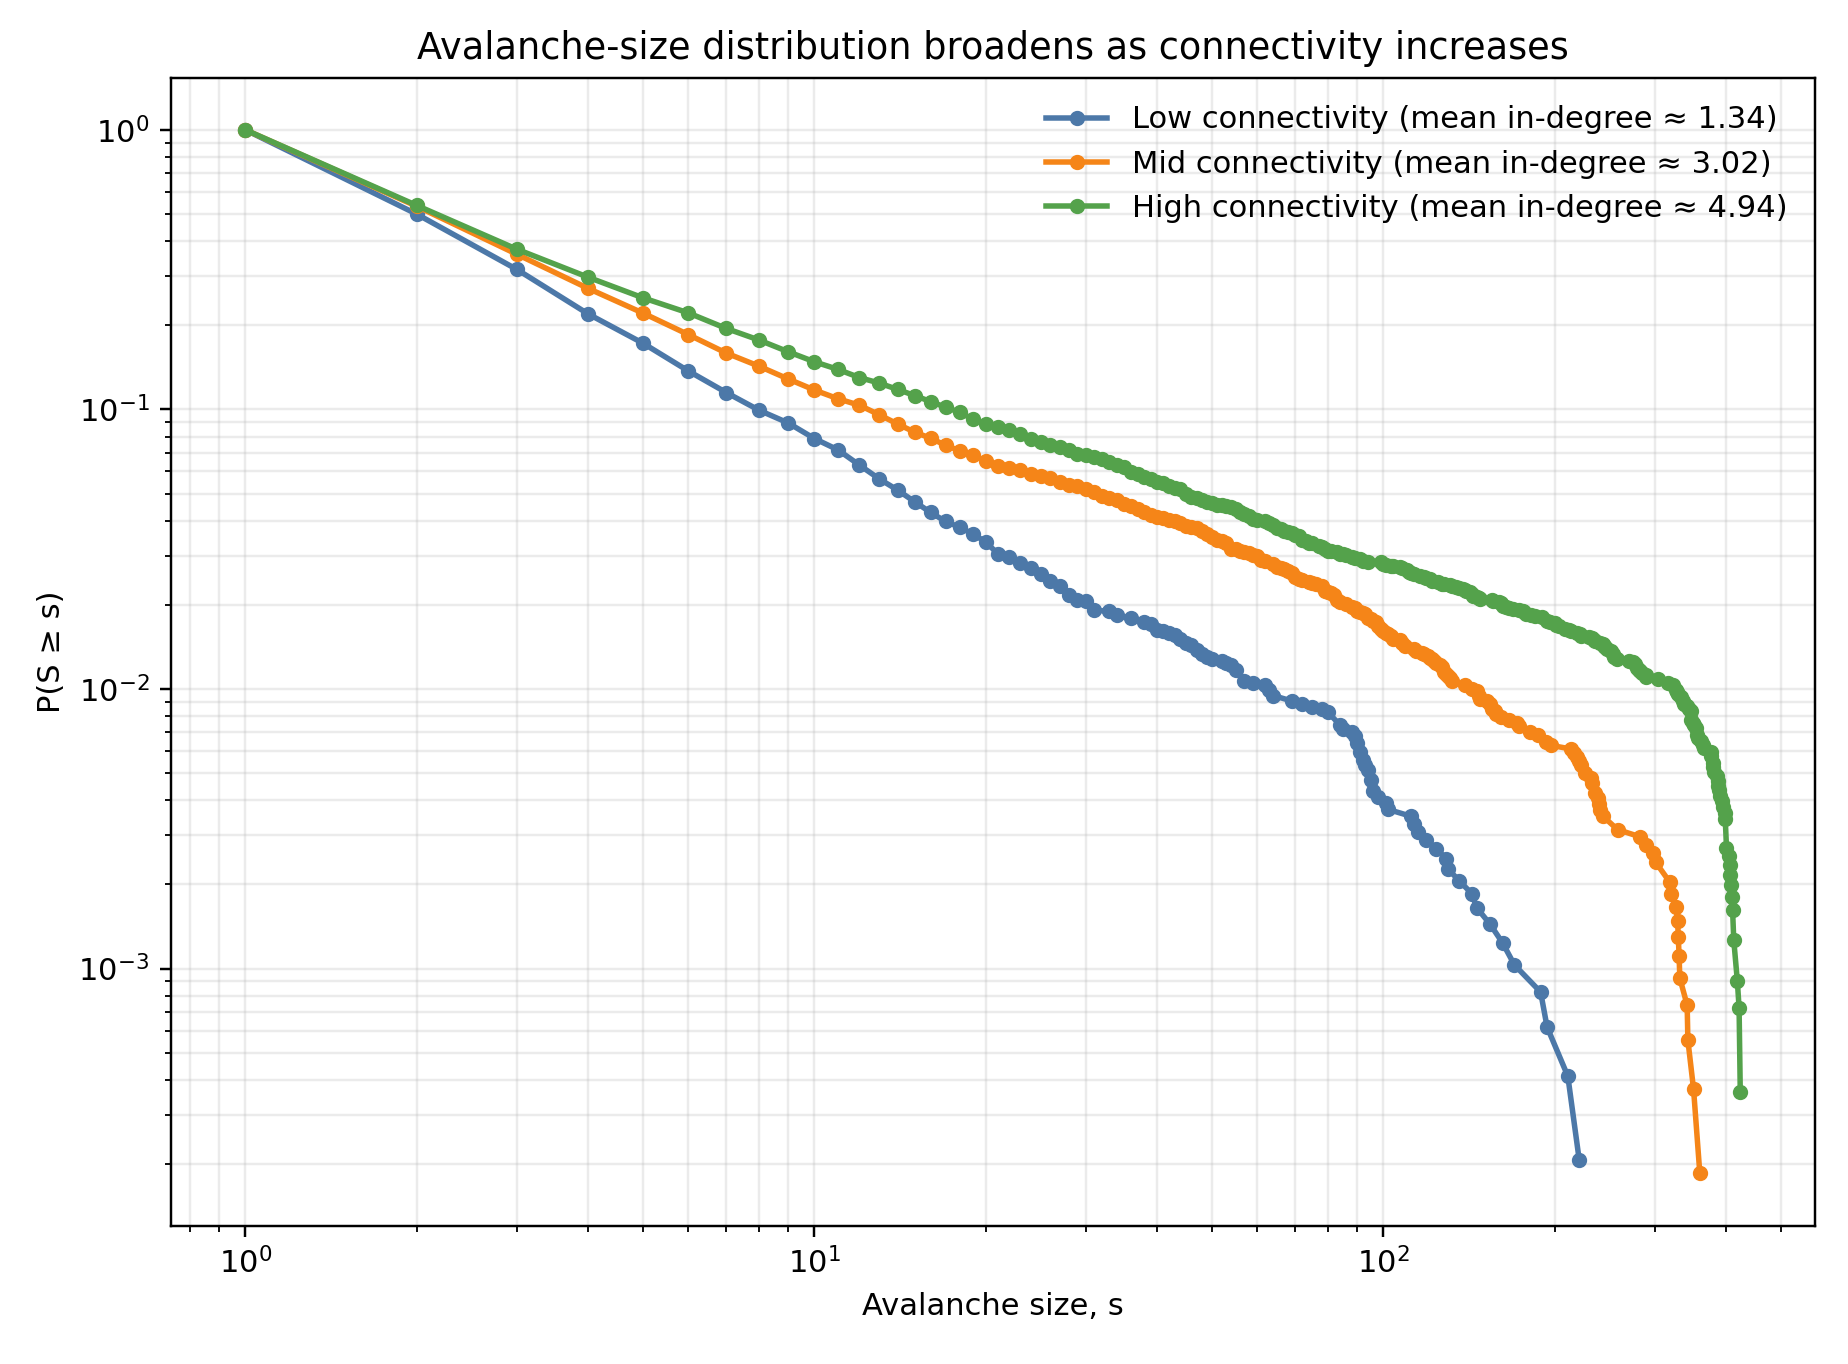
\includegraphics[width=0.82\textwidth]{avalanche_distribution_ccdf.png}
\caption{Avalanche-size distribution broadens with connectivity. The heavier tail at higher connectivity indicates a larger probability of substantial downstream cascades.}
\label{fig:distribution}
\end{figure}

\subsection{Relation Between Avalanche Statistics and Connectivity}
Connectivity has a clear quantitative effect on cascade risk. Table~\ref{tab:summary} summarises the low, medium, and high connectivity cases.

\begin{table}[H]
\centering
\caption{Representative avalanche statistics across connectivity regimes.}
\label{tab:summary}
\begin{tabular}{lcccc}
\toprule
Regime & Mean in-degree & Mean avalanche & 95th percentile & $P(S \geq \LargeAvalancheThreshold)$ \\
\midrule
Low & \ConnectivityLow & \MeanAvalancheLow & \P95AvalancheLow & \LargeProbLow\% \\
Medium & \ConnectivityMid & \MeanAvalancheMid & \P95AvalancheMid & \LargeProbMid\% \\
High & \ConnectivityHigh & \MeanAvalancheHigh & \P95AvalancheHigh & \LargeProbHigh\% \\
\bottomrule
\end{tabular}
\end{table}

The mean avalanche size grows by a factor of \MeanGrowth{} between the lowest and highest connectivity conditions. The probability of a large avalanche increases by \LargeProbChange{} percentage points over the same range, and the largest observed cascade in the highest-connectivity regime affects \HighMaxAvalanche{} downstream libraries. Figure~\ref{fig:connectivity} visualises these trends over the full connectivity sweep.

\begin{figure}[H]
\centering
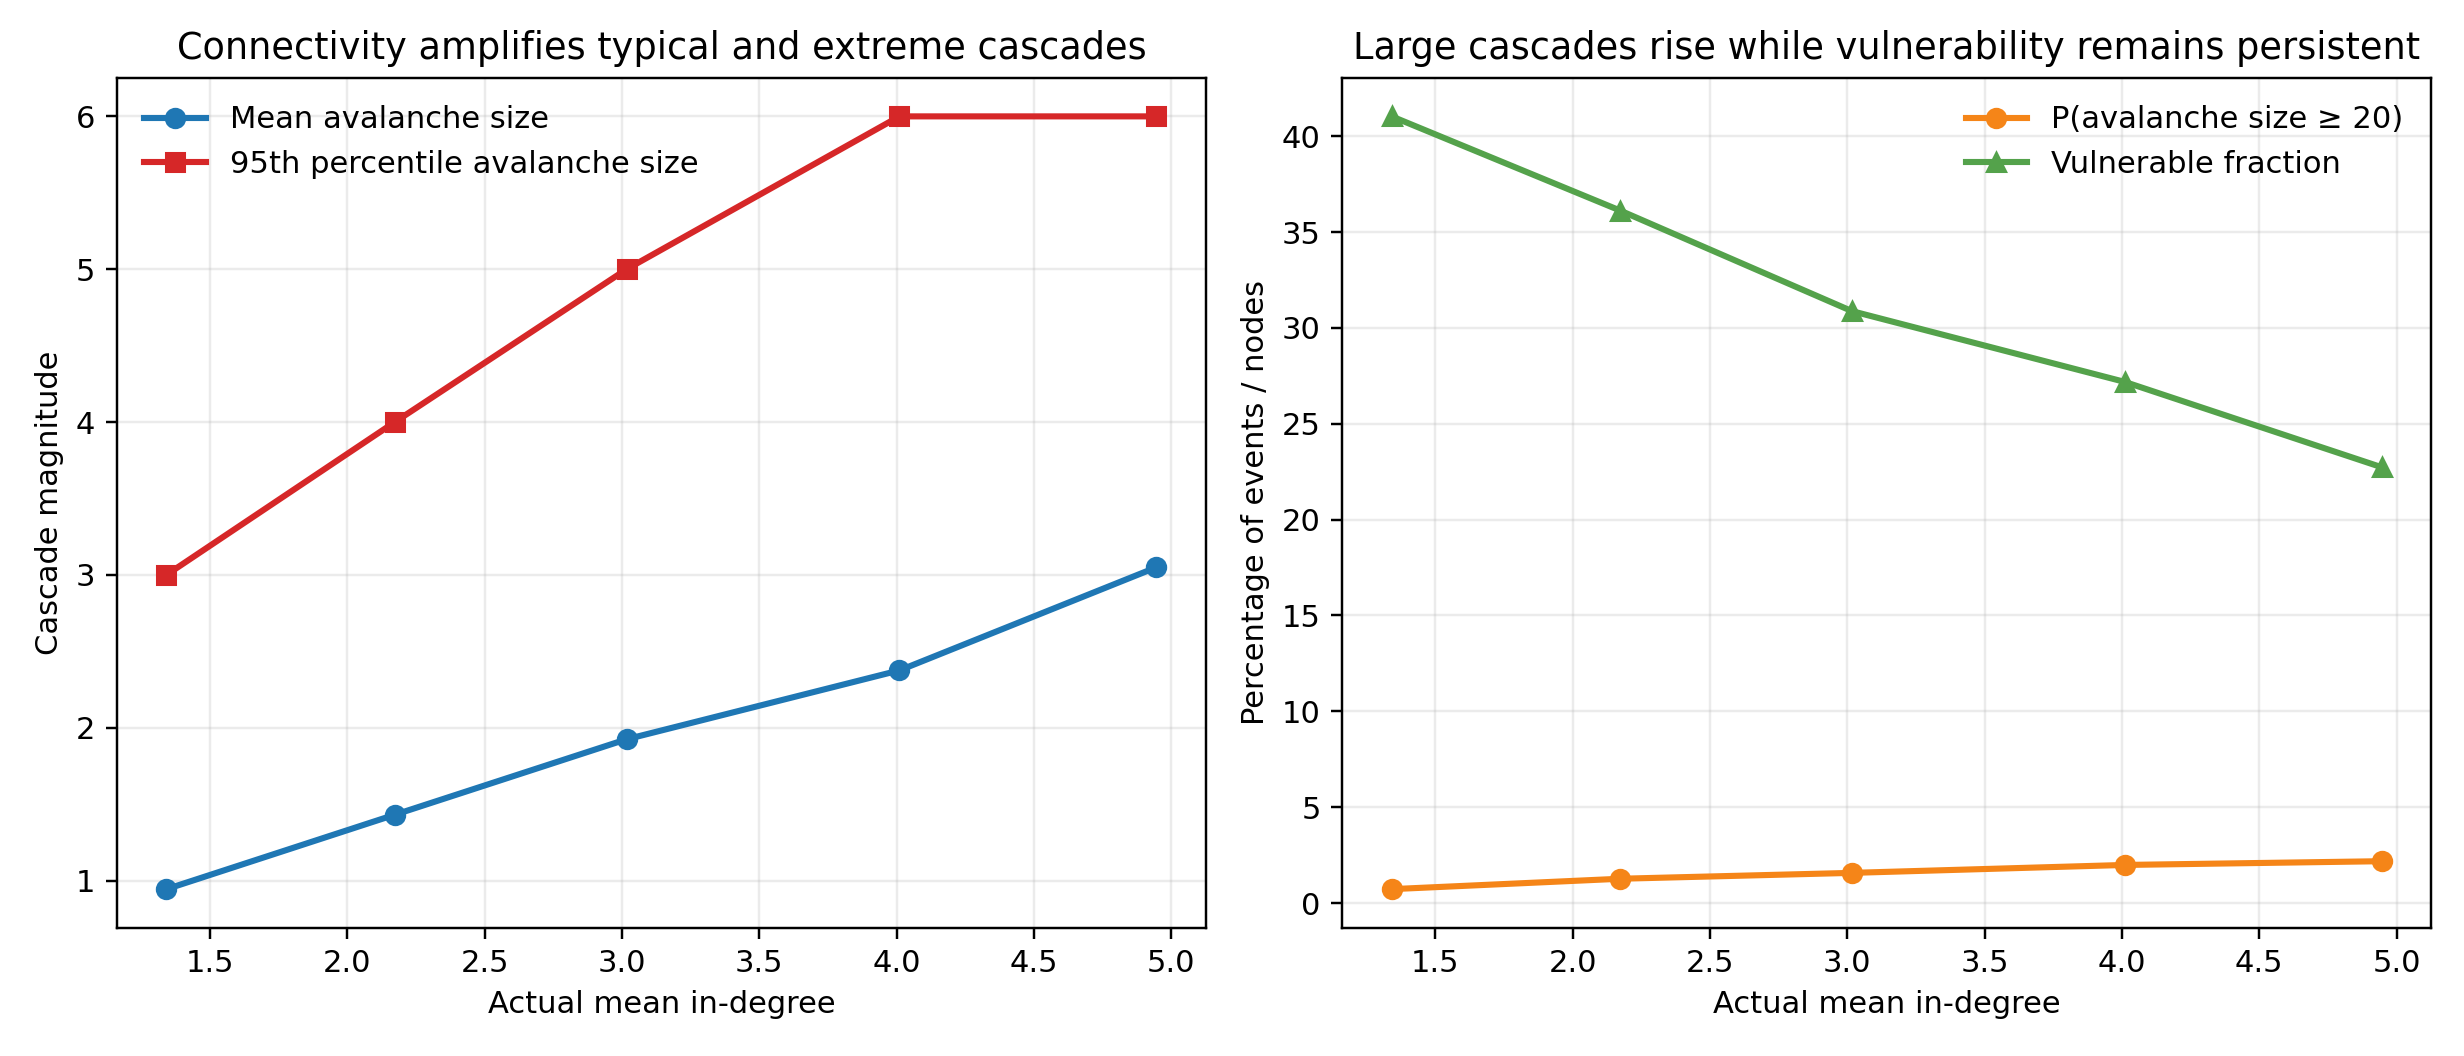
\includegraphics[width=\textwidth]{connectivity_vs_cascade_risk.png}
\caption{Connectivity amplifies both typical and extreme cascade behaviour. As average in-degree grows, mean avalanche size and the probability of large events increase.}
\label{fig:connectivity}
\end{figure}

\subsection{Comment on the Self-Organized Critical State}
The simulation also supports a useful comment on self-organized criticality. The model is slowly driven by isolated updates, but it relaxes quickly through avalanches. Figure~\ref{fig:dynamics} shows that the vulnerable fraction and mean stress ratio settle into a persistent band rather than decaying to zero. In the medium-connectivity regime, about \VulnerableMid{}\% of libraries remain within one additional upstream version increment of failure on average. This indicates that the network self-organizes into a near-threshold state in which large cascades are always possible, even if they are not frequent.

\begin{figure}[H]
\centering
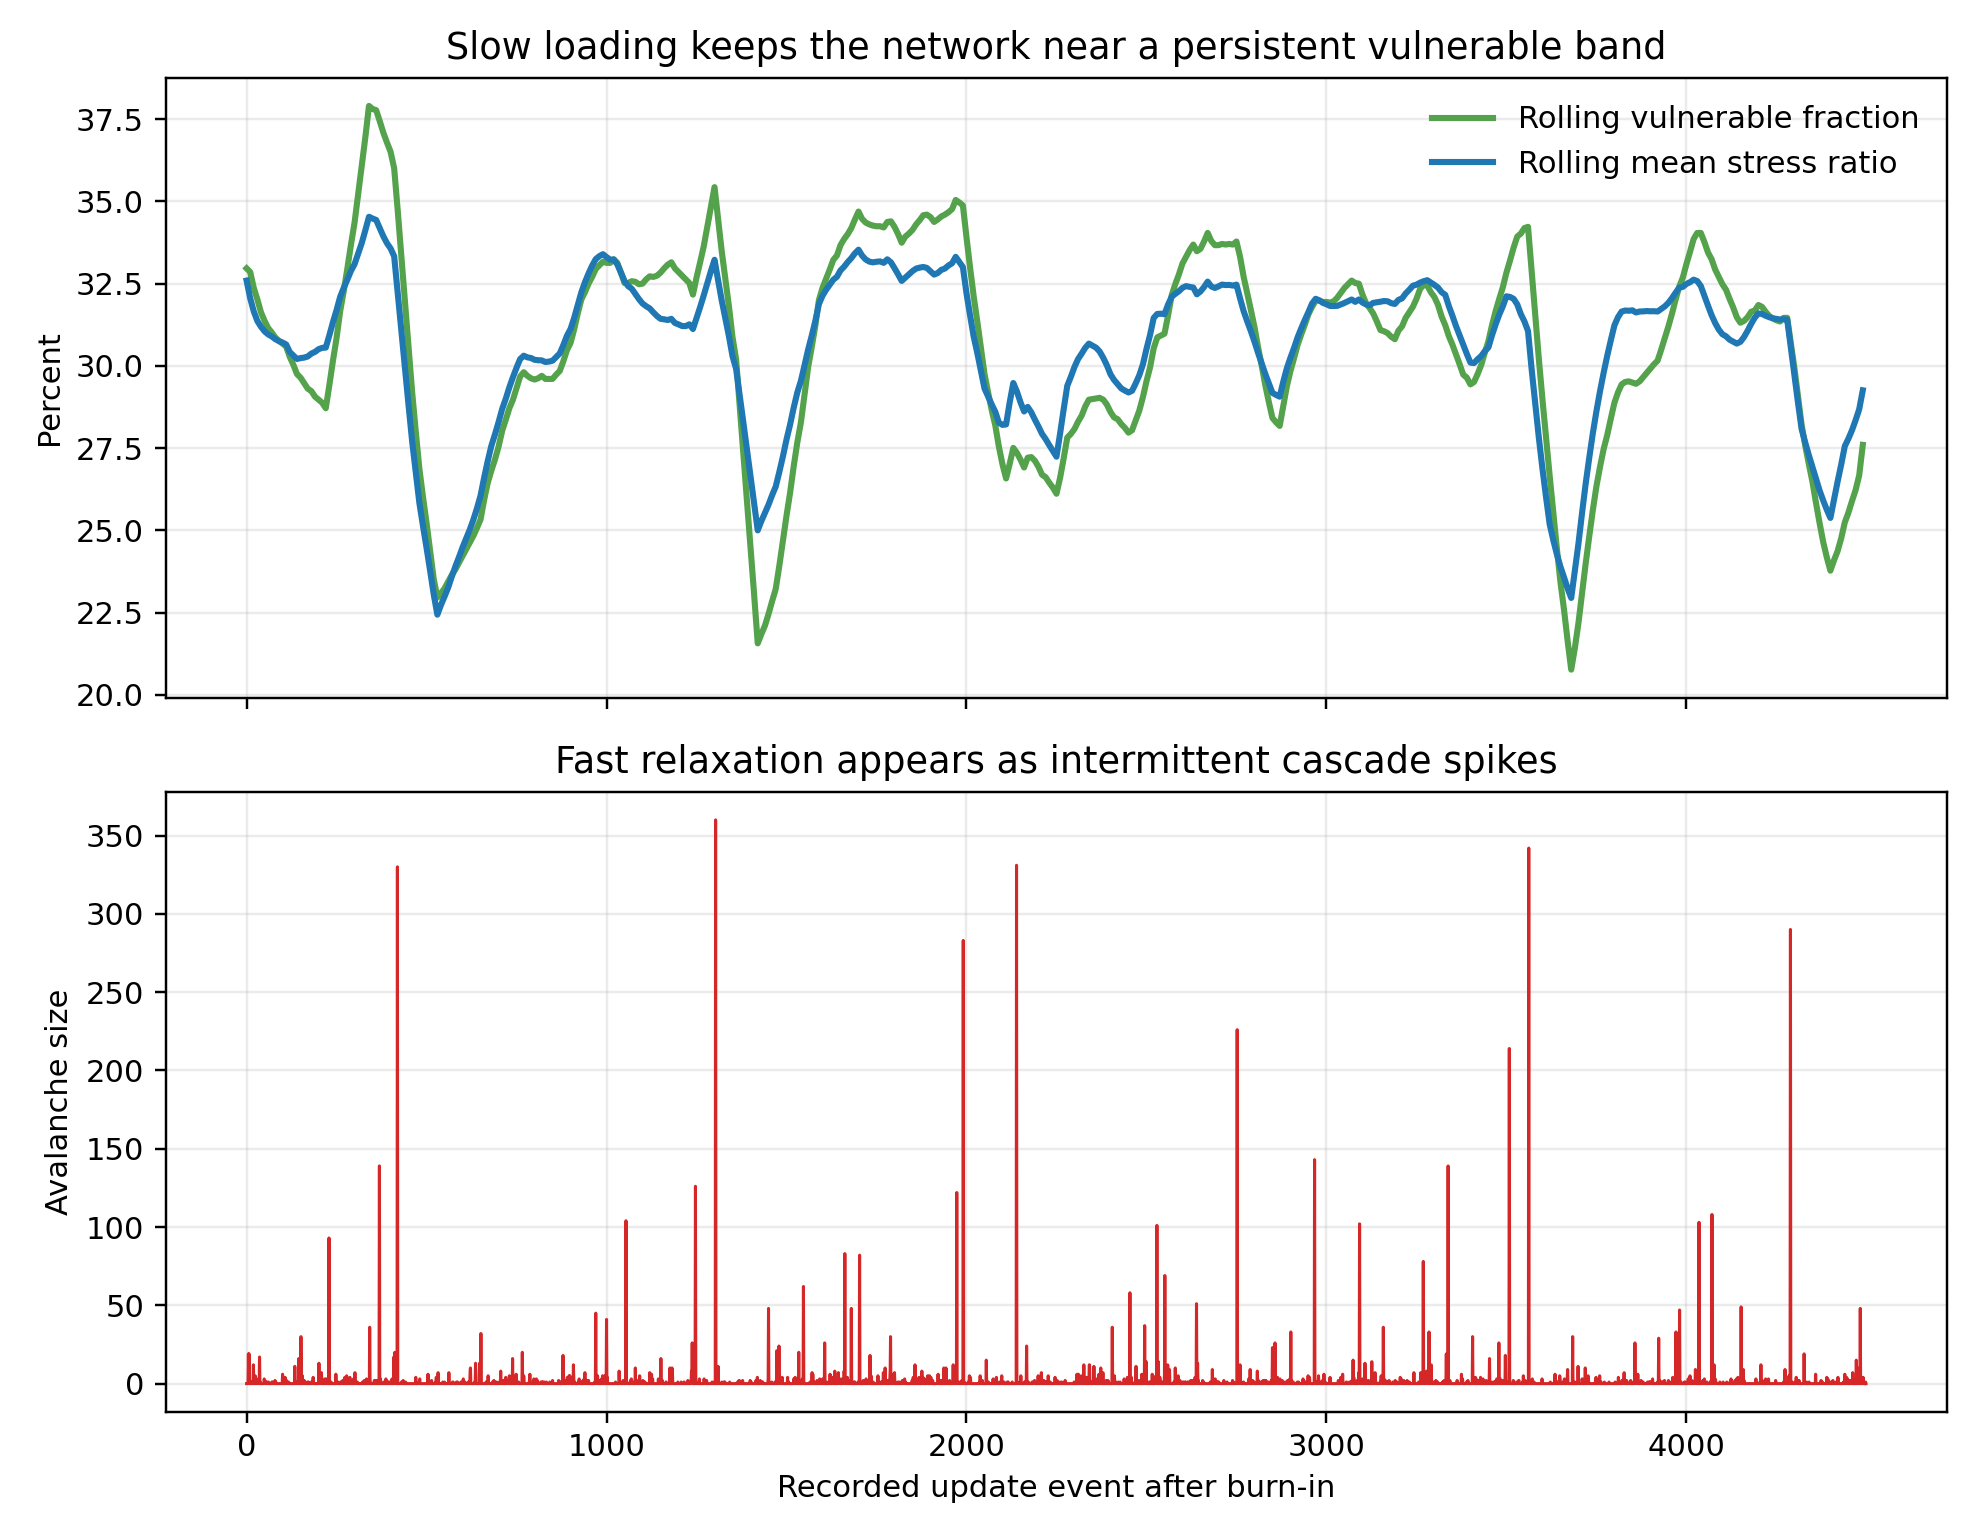
\includegraphics[width=0.92\textwidth]{criticality_dynamics.png}
\caption{Slow loading and fast relaxation in a representative medium-connectivity network. Vulnerability remains persistent while avalanche spikes intermittently release accumulated stress.}
\label{fig:dynamics}
\end{figure}

It would be too strong to claim that this stylised model proves an exact universality class for real software registries. However, it does reproduce the core qualitative hallmarks associated with self-organized critical systems: slow driving, fast dissipation, broad event-size distributions, and a persistent near-critical operating regime \citep{bak1987}.

\section{Discussion}
The simulation suggests that connectivity has a double role. Connectivity improves functionality and reuse by linking packages together, but it also creates more pathways through which breakage can spread. Low-connectivity networks are less efficient in the sense that they share less code, but they are also more resilient to large avalanches. High-connectivity networks are more modular and more powerful, yet they are also more exposed to systemic fragility.

This tradeoff is an important complexity-science insight. The most interesting behaviour does not arise from isolated nodes or fully independent components. It arises when many components are coupled strongly enough that local changes can propagate globally. In that regime, the system exhibits emergent cascade statistics that are not obvious from local package-level reasoning alone.

\section{Conclusion}
This project applied complexity science to a software dependency network, an example outside chemical engineering but highly suitable for complex-systems analysis. The model mapped the assignment requirements directly:

\begin{itemize}[leftmargin=1.4em]
\item random upstream updates acted as noise,
\item downstream breakage cascades acted as avalanches,
\item the dependency graph defined connectivity,
\item simulation quantified the frequency distribution of avalanches and their relation to connectivity,
\item and the persistent near-threshold state supported a meaningful comment on self-organized criticality.
\end{itemize}

The main conclusion is that increasing dependency connectivity increases both the average cascade size and the risk of extreme avalanches. Software ecosystems therefore provide a persuasive and technically rich example of how complexity-science concepts can explain behaviour in socio-technical systems.

\section*{Acknowledgement of Help}
This project used AI assistance for idea development, code drafting, report organisation, and packaging. The simulation outputs, figures, and manuscript included in the repository were generated locally from the included source code. General complexity-science concepts were informed by standard references on complex networks and self-organized criticality.

\section*{Code and Data Availability}
All source code, figures, CSV outputs, and report files are included in the project repository. The repository link can be added after the folder is pushed to a Git-based hosting platform.

\appendix
\section{Prompts Used}
The following prompts were used during project preparation:

\begin{enumerate}[leftmargin=1.4em]
\item Create a complete complexity-science project on software dependency networks, using the assignment requirements and focusing strongly on the simulation and code.
\item Use software dependency networks as the topic, where a random update is the noise and downstream breakage cascades are the avalanches.
\item Build a detailed Python simulation that can study how avalanche statistics depend on network connectivity.
\item Generate publication-style figures, summary tables, and a journal-style manuscript in LaTeX.
\item Include a list of prompts used and acknowledge external help in the report.
\item Package the work so that both the source code and a report PDF are ready for submission.
\end{enumerate}

\bibliographystyle{plainnat}
\bibliography{references}

\end{document}
